\documentclass[tikz,border=4pt]{standalone}
\usepackage{tikz}
\usetikzlibrary{shapes.geometric,arrows.meta,positioning,fit,backgrounds,calc}
\definecolor{argblue}{RGB}{26,79,138}
\definecolor{apsorange}{RGB}{232,119,34}
\begin{document}
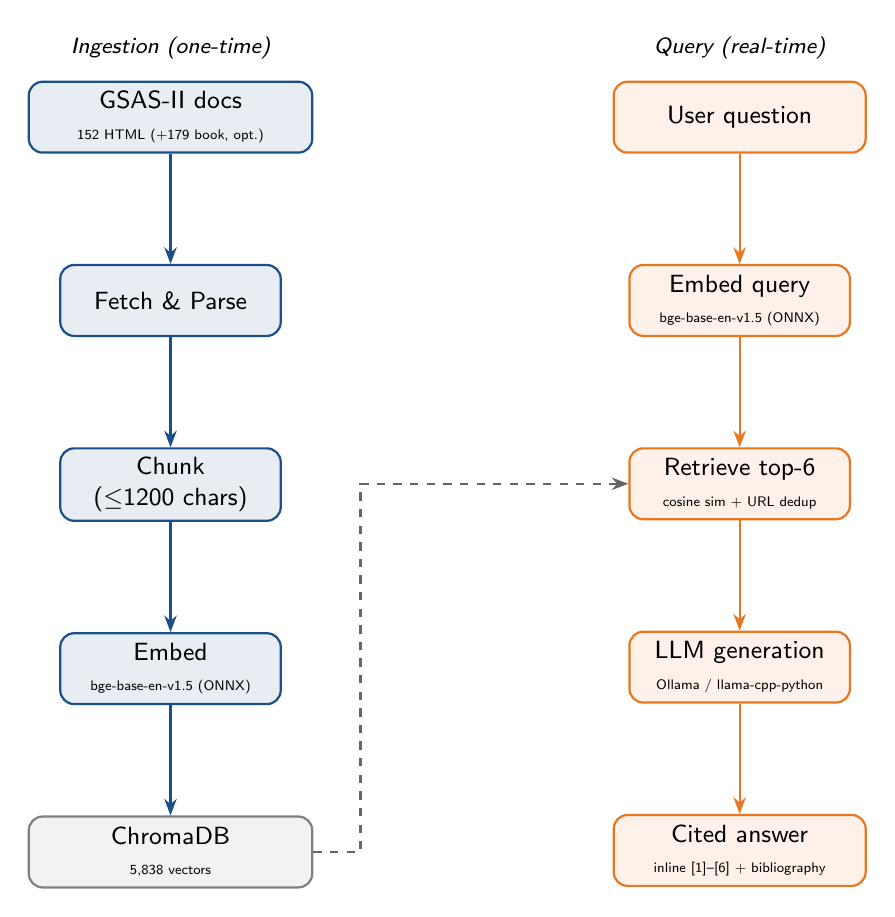
\begin{tikzpicture}[
  node distance = 1.4cm and 2.2cm,
  box/.style  = {rectangle, rounded corners=5pt, draw=#1, fill=#1!10,
                 minimum width=2.8cm, minimum height=0.9cm,
                 font=\small\sffamily, align=center, thick},
  arr/.style  = {-{Stealth[length=6pt]}, thick, #1},
  lbl/.style  = {font=\footnotesize\sffamily\itshape},
]
\node[box=argblue, minimum width=3.6cm] (sources)
  {GSAS-II docs\\{\tiny 152 HTML (+179 book, opt.)}};
\node[box=argblue, below=of sources] (fetch)  {Fetch \& Parse};
\node[box=argblue, below=of fetch]   (chunk)  {Chunk\\($\le$1200 chars)};
\node[box=argblue, below=of chunk]   (embed)  {Embed\\{\tiny bge-base-en-v1.5 (ONNX)}};
\node[box=gray,   below=of embed, minimum width=3.6cm] (chroma)
  {ChromaDB\\{\tiny 5{,}838 vectors}};

\node[box=apsorange, right=3.8cm of sources, minimum width=3.2cm] (user)
  {User question};
\node[box=apsorange, below=of user]    (qembed)  {Embed query\\{\tiny bge-base-en-v1.5 (ONNX)}};
\node[box=apsorange, below=of qembed]  (retrieve){Retrieve top-6\\{\tiny cosine sim + URL dedup}};
\node[box=apsorange, below=of retrieve](llm)     {LLM generation\\{\tiny Ollama / llama-cpp-python}};
\node[box=apsorange, below=of llm, minimum width=3.2cm] (answer)
  {Cited answer\\{\tiny inline [1]\textendash[6] + bibliography}};

\draw[arr=argblue]    (sources) -- (fetch);
\draw[arr=argblue]    (fetch)   -- (chunk);
\draw[arr=argblue]    (chunk)   -- (embed);
\draw[arr=argblue]    (embed)   -- (chroma);
\draw[arr=apsorange]  (user)    -- (qembed);
\draw[arr=apsorange]  (qembed)  -- (retrieve);
\draw[arr=apsorange]  (retrieve)-- (llm);
\draw[arr=apsorange]  (llm)     -- (answer);
\draw[arr=black!60, dashed] (chroma.east) -- ++(0.6,0) |- (retrieve.west);

\node[lbl, above=0.15cm of sources] {Ingestion (one-time)};
\node[lbl, above=0.15cm of user]    {Query (real-time)};
\end{tikzpicture}
\end{document}
